% Yue Li, June 2017

\documentclass[a4paper2pt,twoside]{report}
\usepackage[left=2.5cm,right=2.5cm,top=2cm,bottom=3cm]{geometry}

\usepackage{graphicx}
\usepackage{verbatim}
\usepackage{latexsym}
\usepackage{mathchars}
\usepackage{setspace}
\usepackage[toc]{appendix}
\usepackage{xcolor}
\usepackage{natbib}
\usepackage{hyperref}
\usepackage[labelfont=bf]{caption}
\usepackage[acronym]{glossaries}

\setlength{\parskip}{\medskipamount}  % a little space before a \par
\setlength{\parindent}{0pt}	      % don't indent first lines of paragraphs
%UHEAD.STY  If this is included after \documentstyle{report}, it adds
% an underlined heading style to the LaTeX report style.
% \pagestyle{uheadings} will put underlined headings at the top
% of each page. The right page headings are the Chapter titles and
% the left page titles are supplied by \def\lefthead{text}.

% Ted Shapin, Dec. 17, 1986

\makeatletter
\def\chapapp2{Chapter}

\def\appendix{\par
 \setcounter{chapter}{0}
 \setcounter{section}{0}
 \def\chapapp2{Appendix}
 \def\@chapapp{Appendix}
 \def\thechapter{\Alph{chapter}}}

\def\ps@uheadings{\let\@mkboth\markboth
% modifications
\def\@oddhead{\protect\underline{\protect\makebox[\textwidth][l]
		{\sl\rightmark\hfill\rm\thepage}}}
\def\@oddfoot{}
\def\@evenfoot{}
\def\@evenhead{\protect\underline{\protect\makebox[\textwidth][l]
		{\rm\thepage\hfill\sl\leftmark}}}
% end of modifications
\def\chaptermark##1{\markboth {\ifnum \c@secnumdepth >\m@ne
 \chapapp2\ \thechapter. \ \fi ##1}{}}%
\def\sectionmark##1{\markright {\ifnum \c@secnumdepth >\z@
   \thesection. \ \fi ##1}}}
\makeatother
%%From: marcel@cs.caltech.edu (Marcel van der Goot)
%%Newsgroups: comp.text.tex
%%Subject: illegal modification of boxit.sty
%%Date: 28 Feb 92 01:10:02 GMT
%%Organization: California Institute of Technology (CS dept)
%%Nntp-Posting-Host: andromeda.cs.caltech.edu
%%
%%
%%Quite some time ago I posted a file boxit.sty; maybe it made it
%%to some archives, although I don't recall submitting it. It defines
%%	\begin{boxit}
%%	...
%%	\end{boxit}
%%to draw a box around `...', where the `...' can contain other
%%environments (e.g., a verbatim environment). Unfortunately, it had
%%a problem: it did not work if you used it in paragraph mode, i.e., it
%%only worked if there was an empty line in front of \begin{boxit}.
%%Luckily, that is easily corrected.
%%
%%HOWEVER, apparently someone noticed the problem, tried to correct it,
%%and then distributed this modified version. That would be fine with me,
%%except that:
%%1. There was no note in the file about this modification, it only has my
%%   name in it.
%%2. The modification is wrong: now it only works if there is *no* empty
%%   line in front of \begin{boxit}. In my opinion this bug is worse than
%%   the original one.
%%
%%In particular, the author of this modification tried to force an empty
%%line by inserting a `\\' in the definition of \Beginboxit. If you have
%%a version of boxit.sty with a `\\', please delete it. If you have my
%%old version of boxit.sty, please also delete it. Below is an improved
%%version.
%%
%%Thanks to Joe Armstrong for drawing my attention to the bug and to the
%%illegal version.
%%
%%                                          Marcel van der Goot
%% .---------------------------------------------------------------
%% | Blauw de viooltjes,                    marcel@cs.caltech.edu
%% |    Rood zijn de rozen;
%% | Een rijm kan gezet
%% |    Met plaksel en dozen.
%% |


% boxit.sty
% version: 27 Feb 1992
%
% Defines a boxit environment, which draws lines around its contents.
% Usage:
%   \begin{boxit}
%	... (text you want to be boxed, can contain other environments)
%   \end{boxit}
%
% The width of the box is the width of the contents.
% The boxit* environment behaves the same, except that the box will be
% at least as wide as a normal paragraph.
%
% The reason for writing it this way (rather than with the \boxit#1 macro
% from the TeXbook), is that now you can box verbatim text, as in
%   \begin{boxit}
%   \begin{verbatim}
%   this better come out in boxed verbatim mode ...
%   \end{verbatim}
%   \end{boxit}
%
%						Marcel van der Goot
%						marcel@cs.caltech.edu
%

\def\Beginboxit
   {\par
    \vbox\bgroup
	   \hrule
	   \hbox\bgroup
		  \vrule \kern1.2pt %
		  \vbox\bgroup\kern1.2pt
   }

\def\Endboxit{%
			      \kern1.2pt
		       \egroup
		  \kern1.2pt\vrule
		\egroup
	   \hrule
	 \egroup
   }	

\newenvironment{boxit}{\Beginboxit}{\Endboxit}
\newenvironment{boxit*}{\Beginboxit\hbox to\hsize{}}{\Endboxit}
% Created by Yue Li, June 2017

\pagestyle{empty}

%I commented these out!
%\setlength{\parskip}{0em}
%\setlength{\parindent}{0em}

\makeatletter  %to avoid error messages generated by "\@". Makes Latex treat "@" like a letter

\linespread{1.5}
\def\submitdate#1{\gdef\@submitdate{#1}}
\def\degree#1{\gdef\@degree{#1}}
\def\studentid#1{\gdef\@studentid{#1}}
\def\supervisor#1{\gdef\@supervisor{#1}}

\def\maketitle{
    
  \begin{titlepage}{
    
    \centering{
    
\includegraphics[width=0.5\columnwidth]{images/nottingham-logo.png}} \par
    
    \vskip 1in \par 
    \LARGE {\bf \@title}
    
    \vskip 0.5in \par
    \normalsize {Submitted \@submitdate, in partial fulfillment of \\ the conditions for the award of the degree \bf{\@degree}.}

  }
  \vskip 0.3in \par
  \large {\bf \@author} \par
  \large {\bf \@studentid}
  
  \vskip 0.3in \par
  \large {\bf Supervised by \@supervisor}
  \vskip 0.3in \par
  \normalsize { School of Computer Science \par
  University of Nottingham}

  \vskip 0.5in \par
  \normalsize {I hereby declare that this dissertation is all my own work, except as indicated in the text: }

  \vskip 0.5in 
  \normalsize {Signature 
\includegraphics[]{images/Signature.png}} % \underline{\hspace{1.5in}}
  
  \vskip 0.1in
  \def\mydate{\leavevmode\hbox{\twodigits\day/\twodigits\month/\the\year}}
\def\twodigits#1{\ifnum#1<10 0\fi\the#1}
  \normalsize {Date \mydate} % \underline{\hspace{0.5in}}
  
  %%%%%%%%%%
  %*Only include this sentence below if you do have all necessary rights and consents. For example, if you have including photographs or images from the web or from other papers or documents then you need to obtain explicit consent from the original copyright owner. If in doubt, delete this sentence. See Copyright Information: http://eprints.nottingham.ac.uk/copyrightinfo.html for more details.
  %%%%%%%%%%
  
  \vskip 0.4in \par
  \normalsize {I hereby declare that I have all necessary rights and consents to publicly distribute this dissertation via the University of Nottingham's e-dissertation archive.}

  %%%%%%%%%%
  %Only include this sentence below if there is some reason why your dissertation should not be accessible for some period of time, for example if it contains information which is commercially sensitive or might compromise an Intellectual Property claim. If included, fill in the date from which access should be allowed.
  %%%%%%%%%%

  \vskip 0.4in \par
  \normalsize {Public access to this dissertation is restricted until: \textcolor{red}{DD/MM/YYYY}}
  
  \end{titlepage}
}

\def\titlepage{
  \newpage
  \centering
  \linespread{1}
  \normalsize
  \vbox to \vsize\bgroup\vbox to 9in\bgroup
}
\def\endtitlepage{
  \par
  \kern 0pt
  \egroup
  \vss
  \egroup
  \cleardoublepage
}

\def\abstract{
  \begin{center}{
    \large\bf Abstract}
  \end{center}
  \small
  %\def\baselinestretch{1.5}
  \linespread{1.5}
  \normalsize
}
\def\endabstract{
  \par
}

\newenvironment{acknowledgements}{
  \cleardoublepage
  \begin{center}{
    \large \bf Acknowledgements}
  \end{center}
  \small
  \linespread{1.5}
  \normalsize
}{\cleardoublepage}
\def\endacknowledgements{
  \par
}

\def\preface{
    \pagenumbering{roman}
    \pagestyle{plain}
    \doublespacing
}

\def\body{
	
    \cleardoublepage    
    \pagestyle{uheadings}
    \tableofcontents
    \pagestyle{plain}
    \cleardoublepage
    \pagestyle{uheadings}
    \listoftables
    \pagestyle{plain}
    \cleardoublepage
    \pagestyle{uheadings}
    \listoffigures
    \pagestyle{plain}
    \cleardoublepage
    \pagestyle{uheadings}
    \pagenumbering{arabic}
    \doublespacing
    
}

\makeatother  %to avoid error messages generated by "\@". Makes Latex treat "@" like a letter

% Update \cleardoublepage to be similar in oneside and twoside


\newcommand{\ipc}{{\sf ipc}}

\newcommand{\Prob}{\bbbp}
\newcommand{\Real}{\bbbr}
\newcommand{\real}{\Real}
\newcommand{\Int}{\bbbz}
\newcommand{\Nat}{\bbbn}

\newcommand{\NN}{{\sf I\kern-0.14emN}}   % Natural numbers
\newcommand{\ZZ}{{\sf Z\kern-0.45emZ}}   % Integers
\newcommand{\QQQ}{{\sf C\kern-0.48emQ}}   % Rational numbers
\newcommand{\RR}{{\sf I\kern-0.14emR}}   % Real numbers
\newcommand{\KK}{{\cal K}}
\newcommand{\OO}{{\cal O}}
\newcommand{\AAA}{{\bf A}}
\newcommand{\HH}{{\bf H}}
\newcommand{\II}{{\bf I}}
\newcommand{\LL}{{\bf L}}
\newcommand{\PP}{{\bf P}}
\newcommand{\PPprime}{{\bf P'}}
\newcommand{\QQ}{{\bf Q}}
\newcommand{\UU}{{\bf U}}
\newcommand{\UUprime}{{\bf U'}}
\newcommand{\zzero}{{\bf 0}}
\newcommand{\ppi}{\mbox{\boldmath $\pi$}}
\newcommand{\aalph}{\mbox{\boldmath $\alpha$}}
\newcommand{\bb}{{\bf b}}
\newcommand{\ee}{{\bf e}}
\newcommand{\mmu}{\mbox{\boldmath $\mu$}}
\newcommand{\vv}{{\bf v}}
\newcommand{\xx}{{\bf x}}
\newcommand{\yy}{{\bf y}}
\newcommand{\zz}{{\bf z}}
\newcommand{\oomeg}{\mbox{\boldmath $\omega$}}
\newcommand{\res}{{\bf res}}
\newcommand{\cchi}{{\mbox{\raisebox{.4ex}{$\chi$}}}}
%\newcommand{\cchi}{{\cal X}}
%\newcommand{\cchi}{\mbox{\Large $\chi$}}

% Logical operators and symbols
\newcommand{\imply}{\Rightarrow}
\newcommand{\bimply}{\Leftrightarrow}
\newcommand{\union}{\cup}
\newcommand{\intersect}{\cap}
\newcommand{\boolor}{\vee}
\newcommand{\booland}{\wedge}
\newcommand{\boolimply}{\imply}
\newcommand{\boolbimply}{\bimply}
\newcommand{\boolnot}{\neg}
\newcommand{\boolsat}{\!\models}
\newcommand{\boolnsat}{\!\not\models}


\newcommand{\op}[1]{\mathrm{#1}}
\newcommand{\s}[1]{\ensuremath{\mathcal #1}}

% Properly styled differentiation and integration operators
\newcommand{\diff}[1]{\mathrm{\frac{d}{d\mathit{#1}}}}
\newcommand{\diffII}[1]{\mathrm{\frac{d^2}{d\mathit{#1}^2}}}
\newcommand{\intg}[4]{\int_{#3}^{#4} #1 \, \mathrm{d}#2}
\newcommand{\intgd}[4]{\int\!\!\!\!\int_{#4} #1 \, \mathrm{d}#2 \, \mathrm{d}#3}

% Large () brackets on different lines of an eqnarray environment
\newcommand{\Leftbrace}[1]{\left(\raisebox{0mm}[#1][#1]{}\right.}
\newcommand{\Rightbrace}[1]{\left.\raisebox{0mm}[#1][#1]{}\right)}

% Funky symobols for footnotes
\newcommand{\symbolfootnote}{\renewcommand{\thefootnote}{\fnsymbol{footnote}}}
% now add \symbolfootnote to the beginning of the document...

\newcommand{\normallinespacing}{\renewcommand{\baselinestretch}{1.5} \normalsize}
\newcommand{\mediumlinespacing}{\renewcommand{\baselinestretch}{1.2} \normalsize}
\newcommand{\narrowlinespacing}{\renewcommand{\baselinestretch}{1.0} \normalsize}
\newcommand{\bump}{\noalign{\vspace*{\doublerulesep}}}
\newcommand{\cell}{\multicolumn{1}{}{}}
\newcommand{\spann}{\mbox{span}}
\newcommand{\diagg}{\mbox{diag}}
\newcommand{\modd}{\mbox{mod}}
\newcommand{\minn}{\mbox{min}}
\newcommand{\andd}{\mbox{and}}
\newcommand{\forr}{\mbox{for}}
\newcommand{\EE}{\mbox{E}}

\newcommand{\deff}{\stackrel{\mathrm{def}}{=}}
\newcommand{\syncc}{~\stackrel{\textstyle \rhd\kern-0.57em\lhd}{\scriptstyle L}~}

\def\coop{\mbox{\large $\rhd\!\!\!\lhd$}}
\newcommand{\sync}[1]{\raisebox{-1.0ex}{$\;\stackrel{\coop}{\scriptscriptstyle
#1}\,$}}

\newtheorem{definition}{Definition}[chapter]
\newtheorem{theorem}{Theorem}[chapter]

\newcommand{\Figref}[1]{Figure~\ref{#1}}
\newcommand{\fig}[3]{
 \begin{figure}[!ht]
 \begin{center}
 \scalebox{#3}{\includegraphics{figs/#1.ps}}
 \vspace{-0.1in}
 \caption[ ]{\label{#1} #2}
 \end{center}
 \end{figure}
}

\newcommand{\figtwo}[8]{
 \begin{figure}
 \parbox[b]{#4 \textwidth}{
 \begin{center}
 \scalebox{#3}{\includegraphics{figs/#1.ps}}
 \vspace{-0.1in}
 \caption{\label{#1}#2}
 \end{center}
 }
 \hfill
 \parbox[b]{#8 \textwidth}{
 \begin{center}
 \scalebox{#7}{\includegraphics{figs/#5.ps}}
 \vspace{-0.1in}
 \caption{\label{#5}#6}
 \end{center}
 }
 \end{figure}
}

\makeglossaries
\newacronym{ai}{AI}{Artificial Intelligence}
\newacronym{faq}{FAQ}{Frequently Asked Question}
\newacronym{nlp}{NLP}{Natural Language Processing}
\newacronym{llm}{LLM}{Large Language Model}
\newacronym{cnn}{CNN}{Convolutional Neural Network}
\newacronym{rnn}{RNN}{Recurrent Neural Network}
\newacronym{ann}{ANN}{Artificial Neural Network}
\newacronym{lstm}{LSTM}{Long Short-Term Memory}
\newacronym{gru}{GRU}{Gated Recurrent Unit}
\newacronym{relu}{ReLu}{Rectified Linear Unit}
\newacronym{cbow}{CBOW}{Continuous Bag-of-Words}
\newacronym{gpu}{GPU}{Graphics Processing Unit}
\newacronym{elmo}{ELMo}{Embeddings from Language Model}
\newacronym{bert}{BERT}{Bidirectional Encoder Representations from Transformers}
\newacronym{gpt}{GPT}{Generative Pre-trained Transformer}
\newacronym{glove}{GloVe}{Global Vectors for Word Representation}
\newacronym{squad}{SQuAD}{Stanford Question Answering Dataset}


\begin{document}
\let\cleardoublepage\clearpage % Prevent blank pages being added (otherwise LaTeX ensures new sections start on odd pages....)
\title{Have You Tried Turning It Off and On Again? Pressing reset with a novel framework for the use of deep learning chatbots in education} %Chatbots 2.0: A Novel Framework for Educating the Next Generation

\author{Joel Pointon}
\submitdate{August 2023}
\degree{MSc Data Science}
\studentid{10286413}
\supervisor{Tissa Chandesa}

\normallinespacing
\maketitle

% delete the two declaration sentences in thesis.sty if not applicable. 

\preface
\let\cleardoublepage\clearpage
\addcontentsline{toc}{chapter}{Abstract}

\begin{abstract} %200-500 words

%An abstract (200-500 words) that summarises what the project is about, what it has achieved, and how it contributes to the development of research and/or technology in the area. This should also include  5 to 10 keywords you think would help someone trying to find your dissertation (e.g., in a web search). Please be careful to enter specific keywords relevant to your dissertation, don’t be too general. We recommend that you include full names and acronyms where appropriate, and separate key word with semi-colons e.g. "Keywords: Human Computer Interaction (HCI); Internet of Things (IoT); autonomous vehicles; user study; qualitative study"

Giving a short overview of the work in your project. All code can be found at the following GitHub repository: \url{https://github.com/pointonjoel/MSc-Diss}.

Keywords: \acrfull{ann}; \acrfull{cnn}; \acrfull{nlp}; \acrfull{gpt}; chatbot

\end{abstract}
\cleardoublepage

\addcontentsline{toc}{chapter}{Acknowledgements}

\begin{acknowledgements}

To my beautiful fiancée - the soon-to-be Lily Pointon. You have been my biggest fan and supported me this summer as we prepare for our adventure together! Thank you for listening to me, letting me complain about why things aren't working, and learning enough to write your own dissertation on this... I can't wait for the next stage of life together! 

My unreserved gratitude and thanks go to the spirited and supportive Tissa Chandesa. Your supervision sessions and guidance have been very much appreciated - they inspired this project and helped me to overcome various obstacles.

I also owe Irfan Yaqub many thanks for his expertise and availability to help with debugging and hyperparameter-tuning at various hours of the day. Your assistance has been gratefully received and I wish you all the best with your PhD.

A huge thanks to my future in-laws, Richard and Julianne, for graciously allowing me to check the training progress of my models during mealtimes, and enabling me to work as much as possible during the time I spent in Canterbury. Thanks for welcoming me into your family!

My final thanks go to my wonderful parents, Mum and Dad - your constant support, encouragement and love have helped me get to not only get onto this Master's course, but to thrive on it. Thanks for all your help with planning the wedding and finding a flat, I can't wait to celebrate with you - I love you both!

\end{acknowledgements}

% \printglossaries
% There is a maximum limit of 20,000 words without exceeding 40 pages (A4 sides) for the main body of the dissertation that will be submitted in PDF. This limitation includes the bibliography and excludes cover/front pages (e.g., abstract, acknowledgement, table of contents) and excludes the appendices, listing of any codes or any other supporting documentation.
% Note: Your dissertation should not exceed the word and page limits. You do not have to use up your word limit to get a good grade; never `pad out' your dissertation, this will only annoy the markers.

% Marking criteria:
% A clear statement of the aim of the project?	
% Evidence of knowledge and understanding of context?	
% A convincing motivation of the aim of the project?	
% A clear description of what has been done?	
% Evidence of a suitable technical achievement for a 3 month project?	
% A good evaluation of results?	
% Good technical writing?	
% Overall mark: is it a good dissertation?	
\body
\chapter{Introduction}

% An introduction in which you set out your objectives and briefly introduce the contents of the following chapters to give the reader an overview of what to expect.

% Setting out the aims and objectives of your project, explaining the overall intention of the project and specific steps that will be taken to achieve that intention.

% Motivation and justification are connected with the knowledge and understanding of the context of the project, and also reflect the ability to make good arguments and think critically. A good motivation would be identifying a research gap or unsolved problem; doing something as an exercise to learn some technique or a programming platform is a bad motivation. A good justification for the methodology will be arguing that some technique has never been used to solve the problem, and giving reasons why it may work well for solving it. 

\section{Motivation} %Explaining the problem being solved.
\label{sec:intro_motivation}

In late-2022, ChatGPT was released and left many users speechless at the quality of human-like responses and vast number of possible applications. The mass use of generative chatbots is a new phase in \acrfull{ai}. Rather than simply regurgitating facts from a knowledge base, chatbots can now learn from a corpus of text and generate their own human-like output.

A chatbot is an artificial intelligence system which attempts to simulate human speech in a written manner, without a physical presence \citep{Nee2023ExploringTT}. The increased availability of high-quality, "excellent prose" generative chatbots has several benefits \citep{Floridi}, particularly in education, which this paper will focus on. These include literature review assistance, data analysis, summarisation of documents, and question answering \citep{lund2023chatting}. (ChatGPT was even used to assist in the generation of some BibTeX citations for this paper, to speed up referencing.) However, there are several drawbacks, particularly surrounding perpetuating bias, breaching privacy, and intellectual property rights (not to mention the environmental costs associated with training a \acrfull{llm}) \citep{Jungherr, Bender21}. When it comes to education specifically, generative chatbots pose a heightened possibility of students cheating in assessments, and the inability and unreliability of current methods (and even ChatGPT itself) to detect AI-generated text \citep{susnjak2022, Cotton}.

The increased use of \acrshort{ai} within education is "one of the most important contents of future education development” \citep{BrowMcCoReev2020eu} and is likely to continue to be for many years \citep{zawacki2019systematic}. While there is a need to improve current technology and mitigate the risks and any negative impacts, this paper seeks to focus on the opportunities available to education providers. Historically, Q\&A in the classroom has been difficult and (in higher education) is often constrained to `office hours' or `consultation hours' where lecturers can spend 1-1 time with students to assist with specific queries. However, this can mean that academics repetitively answer similar questions posed by different students. The duplication of questions can be assisted by using platforms such as \citet{Piazza} can enable students to see all queries and post their own anonymously. However, this can also lead to duplicated questions as previous questions and answers are not always seen. Additionally, the professor may need to spend a significant amount of time typing up specific answers. Consequently, there is scope for the learning experience of students to be improved.

There are numerous benefits that chatbots can bring to the classroom \citep{Stanislav}. They can provide answers to \acrshort{faq}s and explain difficult concepts in plain language, which makes them popular among students. Furthermore, students can obtain answers almost instantaneously and at any hour of the day, rather than waiting hours or days for a response from their academic. Furthermore, students' research can be streamlined by pointing them to high-quality sources and finding the most relevant parts, particularly where they may have been overwhelmed by the quantity of information available on search engines \citep{Chen22}. For academics, chatbots can answer the FAQs and more simple, repetitive questions that students have. This can free up academics so that they can spend their time more efficiently, to "reinforce the learning of students", improve their teaching methods \citep{Prez2020}, and "focus on new experimental designs" \citep{Eva}.

However, generative chatbots such as ChatGPT can produce errors \citep{marcus2018, Bender21, Eva}, particularly when seeking to summarise and abstract documents \citep{Durmus_2020}, and can perpetuate any bias in the training data \citep{geva2019, brown2020}. This means that students could be learning inaccurate or irrelevant information. ChatGPT itself, when asked about the drawbacks of chatbots in education, said that ``Chatbots may lack accountability for errors or malfunctions, which could result in incorrect or harmful guidance to students" \citep{chatgpt23}. Additionally, the most advanced chatbots often lack knowledge after a specific date as the training process is computationally expensive and requires a large amount of time \citep{Jungherr}.

\section{Aims and Objectives} %Aims and Objectives here.
\label{sec:intro_aims_and_objectives}

The objective of this paper is to contribute to the field of closed-domain generative question answering. I will seek to discover whether this can be achieved most effectively through fine-tuning a pre-trained model, or through the use of existing fine-tuned models. The overall aim of this paper is to propose an efficient model for academics to create a domain-specific knowledgeable Q\&A chatbot where academics can have high confidence in the accuracy of any answers. Such a platform would be a ``supplement to teaching and learning," rather than replace current teaching methods entirely \citep{Nee2023ExploringTT}. 

%This has been attempted by \citep{Chen22}, using a Deep \acrlong{cnn} (an \acrshort{lstm}-\acrshort{cnn} model). However, a comparison of different models, their training times and practical effectiveness has not been discussed.


\textcolor{red}{ADD RESEARCH QUESTIONS}

%What are my objectives?

\section{Paper Structure}
\label{sec:intro_paper_structure}
%Explaining what your project is meant to achieve, how it is meant to function, perhaps even a functional specification.

This paper will begin by outlining the development of chatbots and the latest state-of-the-art technology used. After this, three potential models will be chosen and justified, the results of their performance will be discussed, and the best-performing model will be outlined. Finally, the findings of this paper will be summarised and complemented by a discussion of the recommended direction of future research. All code can be found at the following GitHub repository: \url{https://github.com/pointonjoel/MSc-Diss}. %against which benchmark?? 

% \textcolor{red}{It's currently being trialed by Khan Academy https://blog.khanacademy.org/harnessing-ai-so-that-all-students-benefit-a-nonprofit-approach-for-equal-access/}
\chapter{Background and Literature Review}

\label{ch:background} 
\label{sec:background}

%A literature and technology review, leading up to the problem that is tackled—you should show a knowledge and awareness of the relevant literature and/or technologies. You shouldn't just give a descriptive list of other work: you should organise the work that you review in an appropriate scheme, show connections and contrasts between the work, point out the strengths and weaknesses of existing work, and where appropriate clearly identify what the current state-of-the-art approaches are to the problem.

Explaining what your project does that is new or is better than existing work in the same field.

\section{Embeddings}
\label{sec:embeddings}

For \acrshort{ai} models to be able to process text, a numerical representation is required. The improvement of these numeric representations has been a key advancement in the area of \acrfull{nlp}, particularly in recent years. Initial models used integer IDs in order to represent words by deriving an integer value from the frequency of a word occuring. This is known as a bag-of-words approach, and is based upon the work of \citet{Zellig}. While there have been variations upon this by using `n-grams' (collections of \textit{n} successive words, this approach is limited in its ability to capture the semantic information within a language \citep{Monisha}. In addition, this method encounters difficulty when the corpus is large and the model dictionary is very large as the model dimensionality is linearly dependent on the number of unique words. 

\subsection{Word2Vec}
\label{sec:embeddings_word2vec}

An alternative approach known as Word2Vec was developed by \citet{mikolov2013efficient} aimed to overcome both of these limitations by building on the work of \citet{bengio2000neural}. It is a technique which uses two-layer neural networks (see Section \ref{sec:background_anns}) in order to produce learned word embeddings, so that words that have similar usage/context in the training corpus are close (have a similar cosine similarity/smallest cosine distance) in the embedding vector space. Therefore, these vectors are superior to integer IDs in containing semantic detail. We can observe this by considering a common example using the vector representations of the words king, man, and woman ($w_K$, $w_M$, and $w_W$ respectively), it can be shown that:
\begin{equation*}
    \begin{aligned}
        w_K - w_M + w_W &\approx w_Q \\
        King - Man + Woman &\approx Queen
    \end{aligned}
\end{equation*}
Where $w_Q$ denotes the vector representation for 'Queen', which is the word with the smallest cosine distance to the above calculation \citep{allen2019analogies}.

\cite{mikolov2013efficient} proposed two possible approaches: one is to use the surrounding words to predict the `current' one (\acrfull{cbow}) and the other is where the `current' word is used to predict the surrounding ones (Skip Gram). A key feature of this approach is that each vector describes the context of the word by considering neighboring tokens, rather than the word itself \citep{li2018introduction}. However, this approach cannot handle words that are not in the training corpus. Additionally, words of opposite sentiment such as “good” and “bad” are closely located in the vector space \citep{sivakumar2020review}, due to the limitations of using a \acrshort{cbow} or Skip Gram approach.

% NOT FOR WORD2VEC: A key benefit of this approach is that vectorised word embeddings have the potential to detect and classify words that are previously unseen to the model \citep{Rudkowsky}.

\subsection{Context}
\label{sec:embeddings_context}

Word2Vec and other similar embeddings such as \acrshort{glove} \citep{Pennington} have long been the industry standard. However, a key limitation is the inability to provide contextualisation. For example, such models provide one vector per word and, as such, they are unable to distinguish between a `fun fair' and a `process being fair', for example. This is because they ignore the ordering of the words and, crucially, simply produce one vector representation per word. Therefore it is essential to generate contextualised embeddings to represent words. Models such as \acrfull{bert} was developed in order by \citet{devlin2019bert} to overcome this limitation, taking into account both left and right context (i.e. words before and after the current word). \textcolor{red}{How do they do this? THIS SEEMS INCOMPLETE/DOESN'T LINK WELL WITH THE NEXT SECTION}.

%(this uses its placement within a sentence using the sin/cos functions? What about the sentence placement - which sentence it is?) Therefore we can have similar representations of fair/unbiased and fair/carnival.

%\acrfull{bert} was developed in order by \citet{devlin2019bert} to overcome this limitation, taking into account both left and right context (i.e. words before and after the current word). Previous models such as \acrshort{elmo} used \acrshort{cnn} and \acrshort{lstm} architecture \citep{peters2018deep}, but \acrshort{bert} dispensed with this technology, using a series of stacked encoders and is trained using masked-language modeling and next sentence prediction. By using Transformers instead of  

%Use BERT's pre-training (Self-supervison) to generate contextual encodings for words? And then use fine-tuning/feature-based approach for use with another model.

%BERT can understand previously unseen/rare words by breaking them into sub-words (`wordpieces') \citep{wu2016googles}.

\section{Early Chatbots}
\label{sec:background_early_chatbots}

The earliest chatbots used rule-based technology to respond to textual inputs. One of the earliest chatbots was Eliza, created in 1966 by researchers at MIT to pass the Turing Test \citep{zemvcik2019}. It used pattern matching to be able to construct human-like replies \citep{Luka}. However, the responses were often formulaic and predictable. Such systems were limited by the complexity of natural language, as it is highly difficult and inefficient to generate rules to handle every possible query. A number of adaptations have been made since these early frameworks, which are outlined below.

%The development of \acrfull{ai} and \acrfull{nlp} meant that chatbots began to learn from data and

\section{\acrlong{ann}s}
\label{sec:background_anns}

\acrlong{ann}s (\acrshort{ann}) are part of a branch of machine learning called deep learning, with machine learning itself being a branch of \acrlong{ai}. \acrshort{ann}s seek to provide solutions to a wide range of classification, pattern recognition and prediction problems, and are used extensively in image recognition and \acrfull{nlp} tasks \citep{Abiodun}. Inspired by the human brain, they are analogous to the nervous system; they take an input and, using a set of complex neurons, seek to identify an output response \citep{Bishop}. They do this by learning from examples, in a similar way to humans. For example, \acrshort{ann}s can be used to predict whether an image contains a pizza or a football.

\subsection{Structure}
\label{sec:background_anns_structure}

Neural networks take a series of inputs (via the input layer) and seek to predict the output (via the output layer). In order to do this, they often contain a number of `fully connected' hidden layers of a pre-determined size that consist of neurons and nodes which themselves contain weights and biases. The size of the input layer is determined by the attributes/information that the model has available to it, and the size of output layer is determined by the classification/prediction problem. 

\begin{figure}[h]
    \centering
    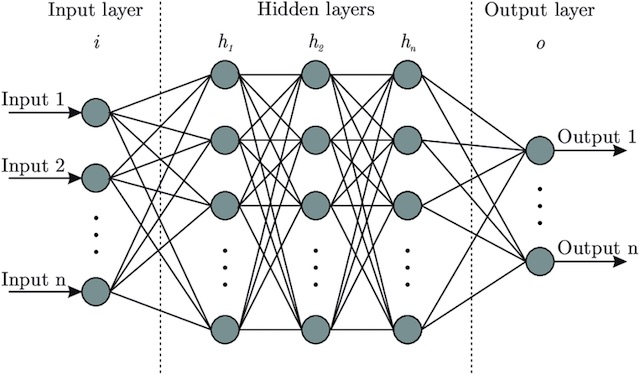
\includegraphics[height=5.5cm] {paper/images/neural_network_structure.jpeg} % ,trim={0 0 0 0cm},clip
    \caption{Typical Neural Network Structure \citep{Shukla}}
    \label{fig:neural_network_structure}
\end{figure}

This structure is shown in Figure \ref{fig:neural_network_structure}, where each grey circle denotes a node, and each interconnecting line denotes a weight between two nodes. As can be seen, each node is connected to every node in the next layer (in a fully connected layer), and the value of each node in the next layer is a weighted sum of the values of the nodes in the previous layer and their corresponding weights (and sometimes a bias term) \citep{Bishop}. The weights therefore determine how much information is passed on to each node in the next layer. The weights are analogous to the strength of connection of biological neurons, and the bias is analogous to the firing threshold.

\subsection{Activation Functions}
\label{sec:background_anns_activation_functions}

The value in each node is of a neural network is typically transformed by an activation function, often Sigmoid or \acrfull{relu}. The former ensures that the values are non-linearly scaled to be between 0 and 1 using $f(x) = \frac{1}{1+e^{-x}}$, whereas the latter truncates values that were below 0 to be 0 using $f(x) = max(0, x)$. Therefore the range of a sigmoid activation function is $(0, 1)$ and the range of a \acrshort{relu} activation function is $[0, \infty]$. These activation functions, along with some other common ones, are shown in Figure \ref{fig:activation_functions}.

\begin{figure}[h]
    \centering
    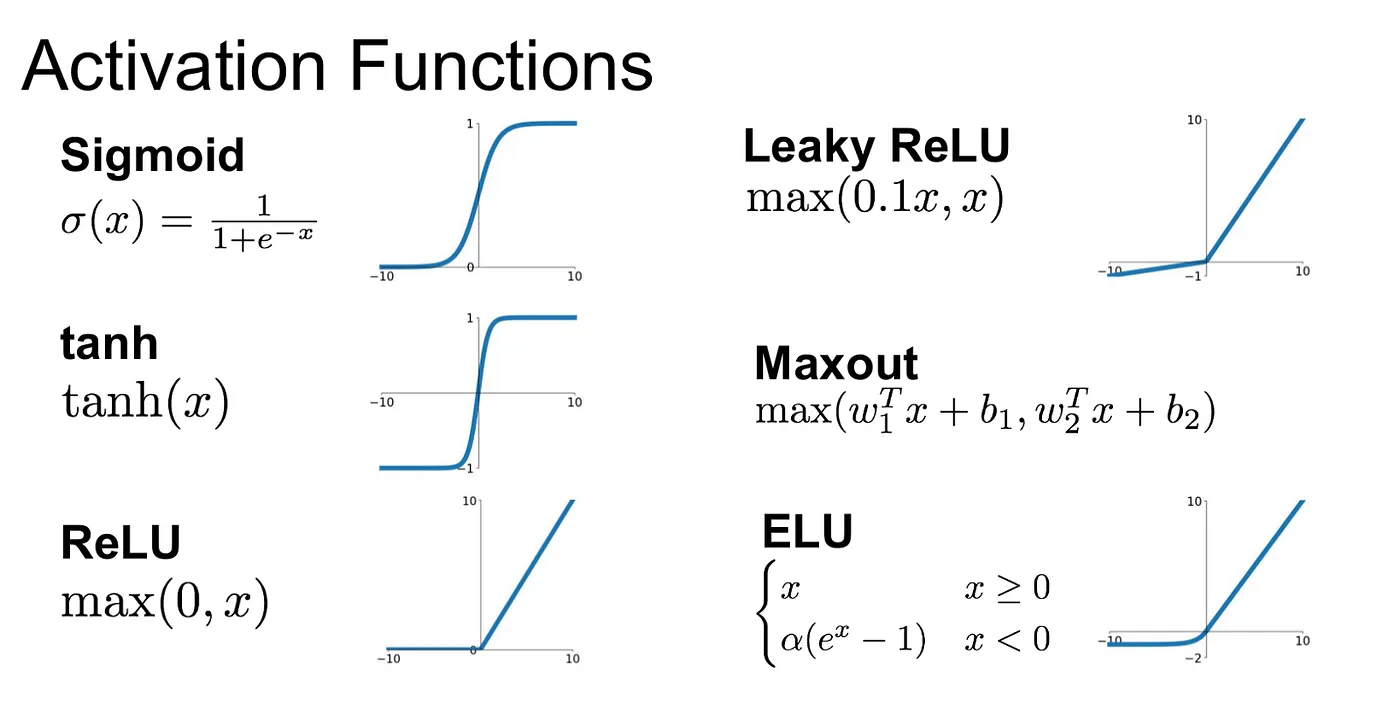
\includegraphics[height=5.5cm,trim={0 0 0 3.5cm},clip]{paper/images/activation_functions.png}
    \caption{Activation Functions used in Neural Networks \citep{Udofia}}
    \label{fig:activation_functions}
\end{figure}

This process is continued for each of the (fully connected) hidden layers, until the network has calculated the values for each of the nodes in the output layer. This will typically be a proportion which, in the case of next sentence prediction, denotes the likelihood of that specific word being the next word in the sentence.

\subsection{Learning}
\label{sec:background_anns_learning}

The learning in neural networks occurs in training the weights that connect each of the nodes. \acrlong{ann}s use a technique known as forward propagation to calculate the predicted output from a given input. Initially, the weights in the network are randomly assigned \citep{Bishop}, meaning that the model has essentially no prior predictive power. For each example data point the network calculates the values for each of the nodes in the output layer; these denote "the probability that the given input fits into each of the pre-set categories" \citep{Yathish}. This process is repeated for each of the training examples, and is known as Forward Propagation. 

The predicted values are subsequently compared against the expected (true) value, and the model and computes the error (the difference between the predicted and true values). This error is fed into a loss function (E), which a measure of the inaccuracy of the model; the aim is to minimise the loss function. For most classification problems, a Cross-entropy (log loss) function is used to compare the difference between the actual value ($y_i$) and the predicted value ($\hat{y_i}$) for each of the prediction classes (N):

$$E = -\sum_i^N y_i*log(\hat{y_i})$$

Once the value for the loss function has been calculated, the model then seeks to update weights and biases in each layer, using a process called Back-propagation \citep{Rumelhart}. We can define the following notation:

$a_j^L$: \textit{The value of the jth note in the Lth layer}

$w_{jk}^L$: \textit{The weight connecting the jth in the Lth layer and the kth note in the (L-1)th layer}

$b_j^L$: \textit{The bias applied to the jth note in the Lth layer}

$z_j^L = w_j^L a_j^{L-1} + b_j^L$: \textit{The value of the jth note in the Lth layer}

We can therefore say that $a_j^L = \sigma(z_j^L)$, where $\sigma$ denotes the activation function.

Backpropagation process begins by computing the rate of change of the cost function with respect to each of the weights (holding other weights constant) because we are seeking to minimise the cost function. This is given by:
$$\partial E/ \partial w_{jk}^L,\quad \forall  i \in [1,n^L]$$ where $n^L$ denotes the size of the current layer. By using the chain rule, we can expand this:
$$\frac{\partial E}{\partial w_{jk}^L} = \frac{\partial z_j^L}{\partial w_{jk}^L} \frac{\partial a_j^L}{\partial z_j^L} \frac{\partial E}{\partial a_j^L}$$ % \; can work for spacing
Similarly, we can calculate $\partial E/ \partial b_j^L$ and $\partial E/ \partial a_j^{L-1}$. Using these, the gradient of the cost function can be computed, and used to update the parameters above so that the cost function is reduced. Gradient Descent is the process of adjusting the parameters in the `direction' indicated by the gradient of the cost function, such that the loss function is reduced. The size of adjustment is called the `learning rate', and this affects how quickly the model adjusts its parameters.

This adjustment is applied to all of the network's layers as part of the backpropagation process, and for each of the training examples. One iteration of the combined training process is known as an Epoch (Forward Propagation, Cost Calculation, and Backpropagation using Gradient Descent) \citep{Sharma}, and this is applied recursively until the loss function is sufficiently small. The smaller the learning rate, the more epochs are typically required to reach the minimum loss required. Once all of the epochs are completed, the model has finished training and it has achieved the parameters which give optimal predictions.

\section{\acrlong{rnn}s}
\label{sec:background_rnns}

\acrlong{rnn}s are a form of neural network used for sequential data. They take each element of the sequence one at a time and use the current and previous values to predict future ones. They can crudely be thought of as ``very deep feedforward networks in which all the layers share the same weights'' \citep{Yann}. This is depicted in Figure \ref{fig:rnn_architecture}, where the input is processed sequentially ($x_{t-1}, x_{t}, x_{t+1},\ldots$), and information from the previous state is used to make the prediction in the current state ($h_{t}$). However, when backpropagation is used to train the network, problems are often encountered.

\begin{figure}[h]
    \centering
    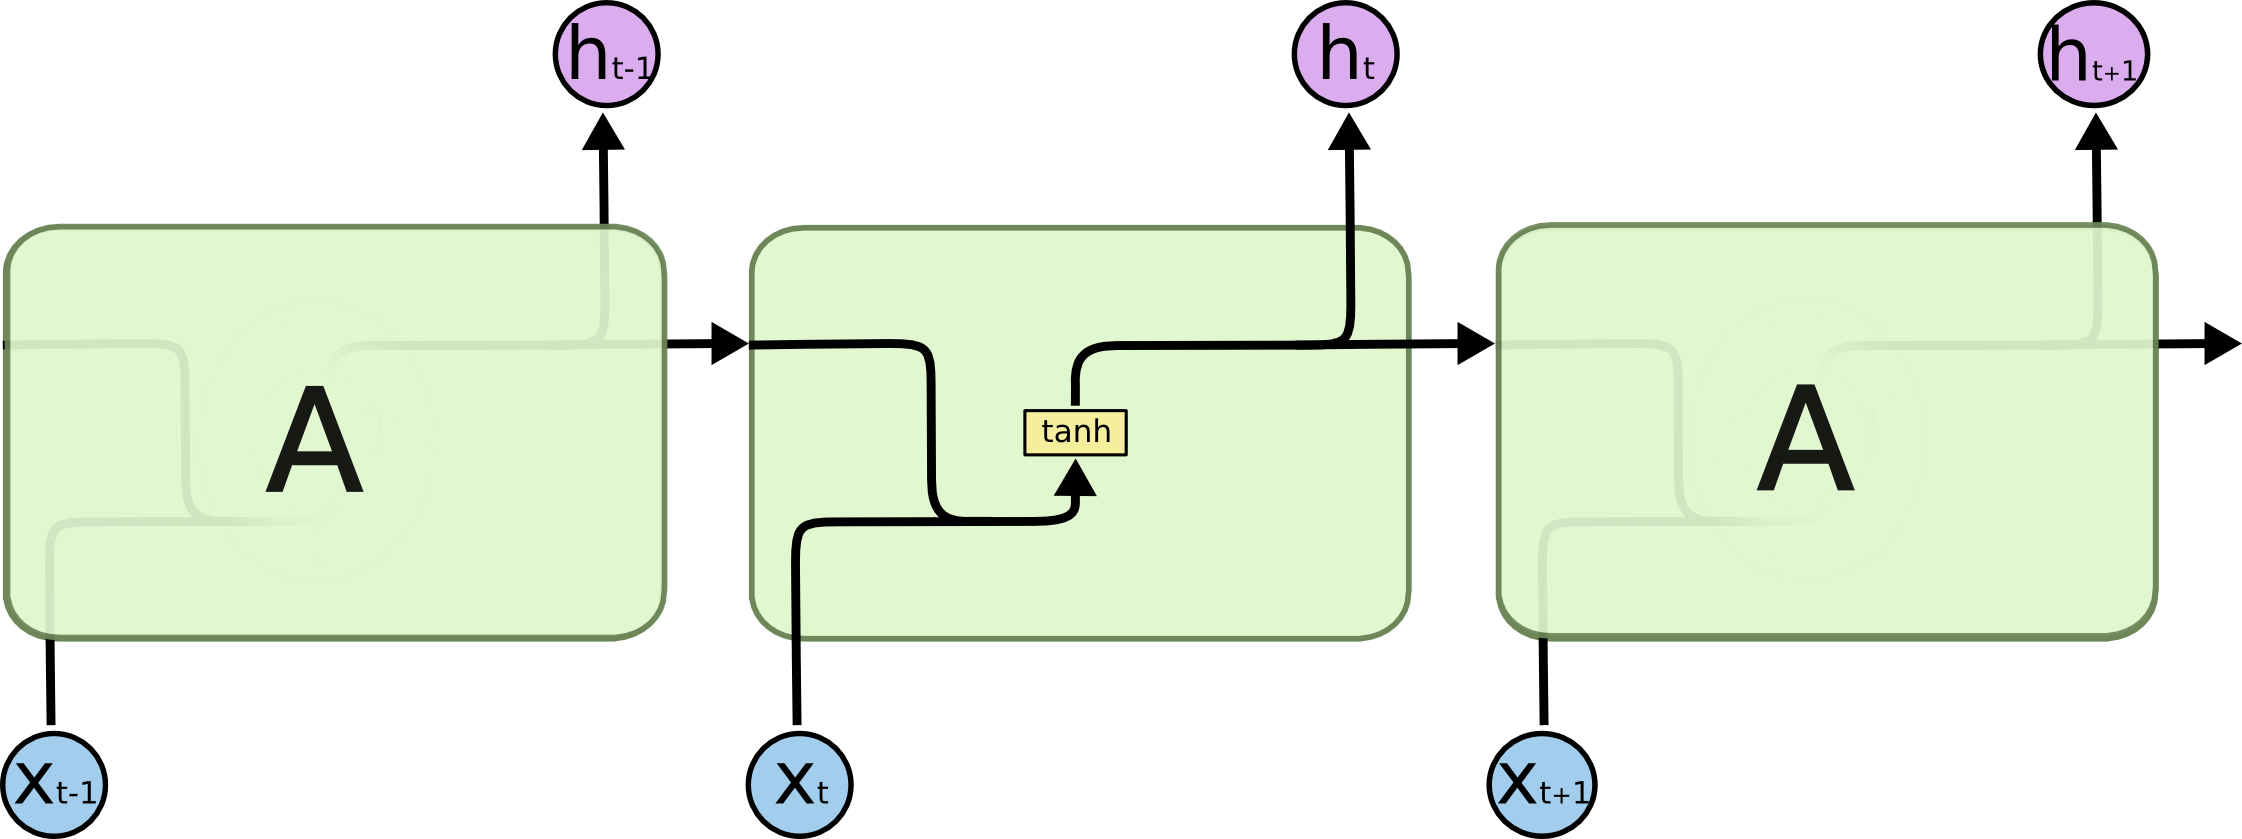
\includegraphics[height=4.5cm,trim={0 0 0cm 0cm},clip]{paper/images/rnn.png}
    \caption{Architecture of a \acrlong{rnn} \citep{olah2015understanding}}
    \label{fig:rnn_architecture}
\end{figure}

A common problem with training neural networks is the vanishing/exploding gradient problem \citep{hochreiter1997long}. This can occur in deep neural networks but is particularly common in \acrshort{rnn}s, as the same weights are used in each iteration. The exploding gradient problem is where the model weights become exponentially large, which causes the model weights to become NAN. Alternatively, because of the recurrent structure of the model, there can be a tendency for model weights to `vanish' and tend to 0. This causes the model to have short-term memory because it fails to capture long-term dependencies \citep{chung2014empirical}. In addition to this, in both cases, the loss function is not minimised because the weights cause the loss function to either overshoot or never reach the global/local minimum.

\subsection{\acrlong{lstm} Cells}
\label{sec:background_lstms}

\acrshort{lstm} networks are a type of \acrlong{rnn} which were developed by \citet{hochreiter1997long} in order to overcome the vanishing/exploding gradient problem. They are depicted in Figure \ref{fig:lstm_architecture} where, instead of one simple layer (as in Figure \ref{fig:rnn_architecture}), there are 3 layers with different activation functions. \acrshort{lstm} networks use sigmoid ($\sigma$) a activation function for each of its 3 `gates' (forget gate, input gate, and output gate) to determine how much of the long-term memory is maintained and to update both the long-term and short-term memory in each cell. The first (most left-wise neural network layer in Figure \ref{fig:lstm_architecture} is the `forget gate'. The `input gate' refers to the second layer, which is subsequently combined with a layer with a tanh activation function to update the long term memory. The final layer is the `output gate', and also uses a sigmoid activation function. By using this structure, \acrshort{lstm} networks overcome the vanishing and exploding gradient problem because they control how much the gradient vanishes using the `forget gate' \citep{Gers}.

\begin{figure}[h]
    \centering
    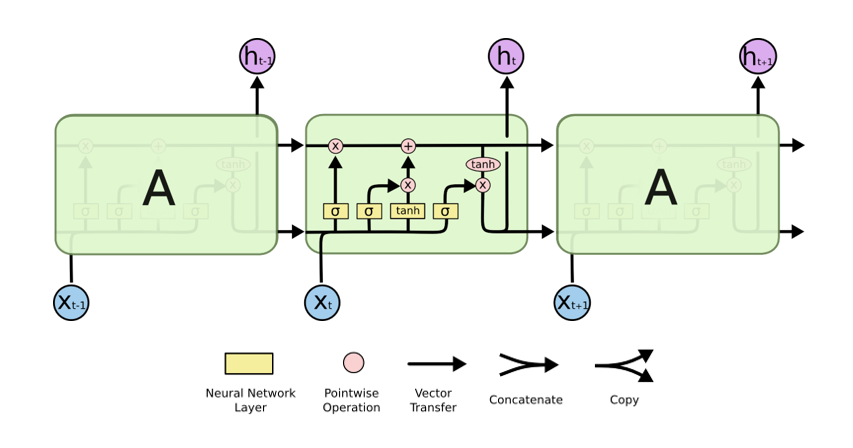
\includegraphics[height=7.5cm,trim={0 0 0 0cm},clip]{paper/images/lstm.png}
    \caption{Architecture of a \acrlong{lstm} cell \citep{olah2015understanding}}
    \label{fig:lstm_architecture}
\end{figure}

\subsection{\acrlong{gru}s}
\label{sec:background_grus}

Another similar model to \acrshort{lstm}s is the \acrfull {gru}, with an architecture based on just two gates (reset gate and update gate). It was developed in 2014 by \citet{cho2014learning} and provides a simpler architecture than the \acrshort{lstm} model. This model is shown in Figure \ref{fig:gru_architecture}, which shows how the flow of information is held using a `hidden state' and the two gates (the neural network layers with sigmoid activation functions) determine how much information it remembers or forgets. The update gate determines how much of the memory it retains, and the reset gate determines how much of the memory it forgets.

\begin{figure}[h]
    \centering
    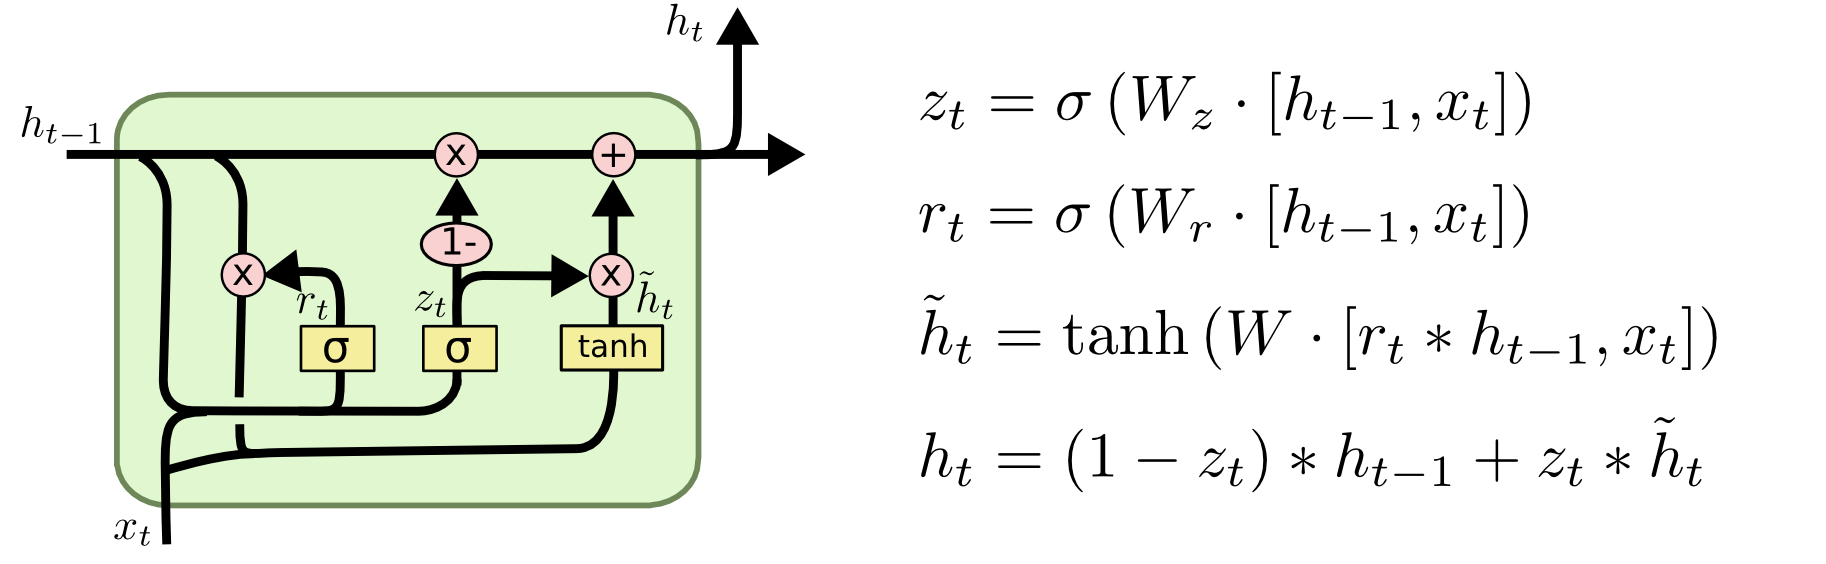
\includegraphics[height=4.5cm,trim={0 0 12cm 0cm},clip]{paper/images/gru.png}
    \caption{Architecture of a \acrlong{gru} \citep{olah2015understanding}}
    \label{fig:gru_architecture}
\end{figure}

The \acrlong{gru} has become popular due to its simplicity relative to the \acrshort{lstm} architecture, but \acrlong{lstm} cells and \acrlong{gru}s often perform similarly effectively. However, it has been noted in the literature that \acrshort{gru}s generally outperform LSTM networks on sequences that are short and less complex, whereas \acrshort{lstm} models are typically favoured for longer and more complex sequences \citep{cahuantzi2023comparison}. This is often attributed to the \acrshort{lstm} model's ability to better capture long-term dependencies in sequences, which often means it is preferred for language modelling \citep{Irie2016}. However, both models can only capture forward dependencies, due to their sequential nature. For example, with the sentence `Joel read a book about a bass that was owned by a fisherman', using only the first 7 words, you would not know whether the word `bass' refers to the fish or the instrument. It is only with the latter parts of the sequence that you can determine the context and therefore the bass was owned by the fisherman and not the musician. Therefore, models which only capture forward dependencies will miss any potential inference based on future words. 

\subsection{Bidirectional \acrlong{rnn}s}
\label{sec:background_bidirectional_rnns}

To overcome this limitation, Bidirectional \acrshort{rnn}s were developed by \citet{Schuster} and are a combination of two \acrshort{rnn}s (Section \ref{sec:background_rnns}). One processes information in the usual chronological manner, with a second processing it in reverse time order. The model is trained simultaneously on both of these and seeks to minimise the loss function for both time directions concurrently. This allows the model to capture the future context in sequences, which is particularly important in \acrshort{nlp} implementations because the context of words is typically derived from future words.

All of the above models (\acrshort{rnn}s, \acrshort{lstm}s, and \acrshort{gru}s) require sentences to be processed sequentially, and so can take a long time to train especially when there are long strings to process, and can have convergence issues due to vanishing/exploding gradients \citep{vaswani2017attention, Lipton}. We will now explore 2 alternative models which seek to solve this.

\section{\acrlong{cnn}s}
\label{sec:background_cnns}

A popular varation of the vanilla neural network is the \acrfull{cnn}. It uses convolutions for feature extraction which is then fed into a fully connected neural network for the classification \citep{Budiharto}, and is efficient as convolutions perform well on \acrshort{gpu}s. They have been used to produce \acrfull{sota} results in image classification \citep{krizhevsky2017imagenet}, but can also be successfully applied to \acrshort{nlp} tasks \citep{kim2014convolutional}.

The architecture is outlined in Figure \ref{fig:cnn_architecture}. The model begins by convolving multiple matrix filters over the concatenated vector representation of the input sequence (often word2Vec; see Section \ref{sec:embeddings_word2vec}) in order to extract
patterns in the input. Each convolutional layer typically contains a non-linear activation function (Section \ref{sec:background_anns_activation_functions}), after which pooling is used to reduce dimensionality without losing the most important information \citep{Severyn2015UNITNTD}. Typically, max pooling is used. The final layer is a fully connected softmax layer which outputs the probability distribution of the various output classes (e.g. sentence sentiment).

\begin{figure}[h]
    \centering
    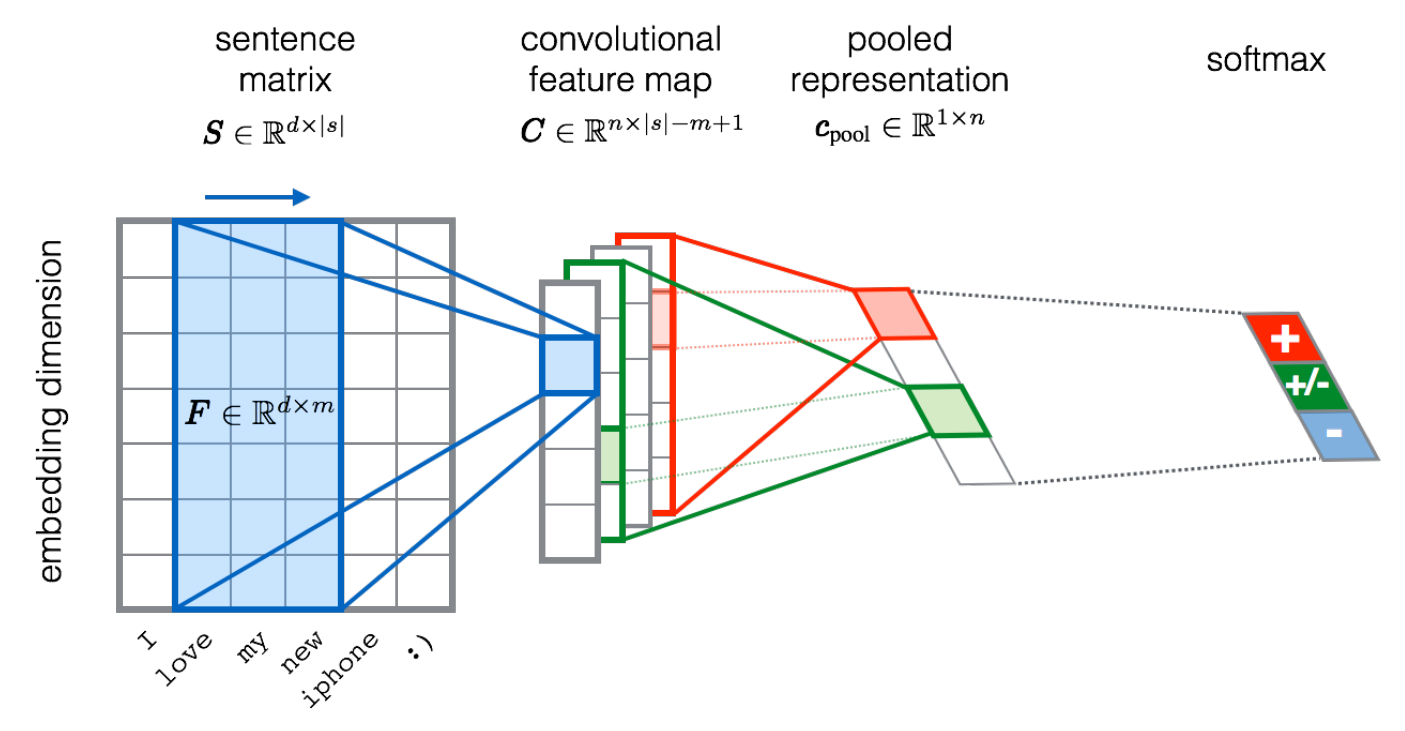
\includegraphics[height=6cm,trim={0 0 0cm 0cm},clip]{paper/images/cnn.png}
    \caption{Architecture of a \acrlong{cnn} \citep{Severyn2015UNITNTD}}
    \label{fig:cnn_architecture}
\end{figure}

%Deep learning is a subfield of Machine Learning, with vast applications, particularly within computer vision and \acrshort{nlp}.

\section{Transformers}
\label{sec:background_transformers}
Transformers were introduced in \citeauthor{vaswani2017attention}'s 'Attention Is All You Need' paper (\citeyear{vaswani2017attention}). The authors proposed a sequence-to-sequence model which uses $N=6$ stacked encoders and decoders (although subsequent models use varying numbers of encoders and/or decoders). The strength of Transformers lies in their ability to process all words a sentence simultaneously (the sequential nature of \acrshort{lstm} networks made them slow to train), and their ability to retain context from much further back in the sequence \cite{vaswani2017attention}. 

While there are many variations, the initial model architecture is shown in Figure \ref{fig:transformer_architecture}. It begins by taking initial embeddings (learned embeddings such as word2Vec - Google's \acrshort{bert} uses wordpiece tokenisation in order to easily handle out-of-vocabulary words \citep{wu2016googles}), and applies a vector containing positional encodings for each word (using $sin$ and $cos$ functions). These positional encodings are then passed into the encoder block.

\begin{figure}[h]
    \centering
    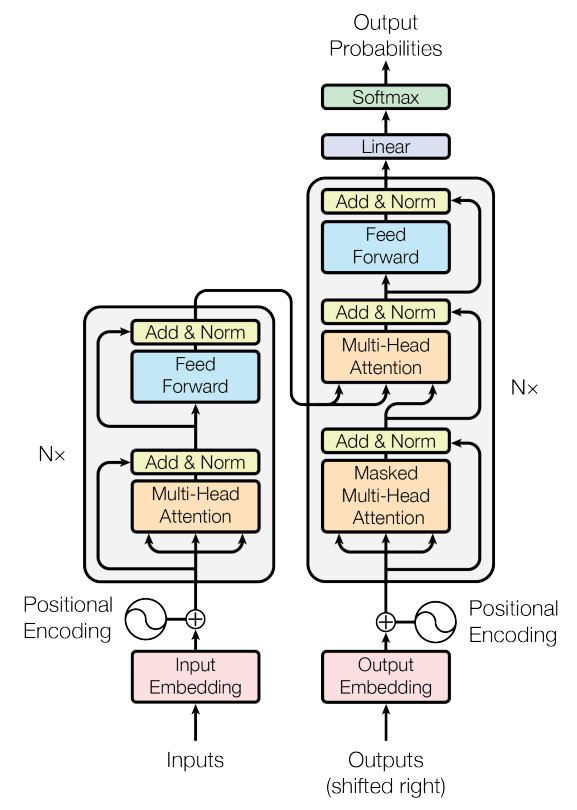
\includegraphics[height=10cm,trim={0 0 0cm 0cm},clip]{paper/images/transformer.png}
    \caption{Architecture of a Transformer model \citep{vaswani2017attention}}
    \label{fig:transformer_architecture}
\end{figure}

\subsection{Encoder}
An encoder consists of a multi-headed attention block combined with a feed-forward neural network, both of which are followed by layer normalisation. Firstly, the positional encoding vectors are used to calculate self-attention vectors, which specifies how each word relates to every other word in the sequence. Each of the self-attention vectors can be passed into the neural network independently of each other, meaning that the model can take advantage of the parallelisation offered by \acrshort{gpu}s, reducing training time. Finally, the encoder outputs a contextualised vector, which can be intuitively conceptualised as containing the `meaning' of the word within its context.

\subsection{Decoder}
The decoder uses a similar architecture to the encoder, but uses masking to prevent the model from `seeing ahead' in the sentence. For example, to translate the phrase ``Esta es una tesis fantástica'' from Spanish to English, the model should not see any word ``tesis fantástica'' when calculating the self-attention for the phrase ``Esta es una''. This means that the model has unidirectional-context (typically only left-context). Once the masked multi-headed attention vectors have been calculated, the decoder combines this with the output from the encoder using another multi-headed attention block. Finally this information is passed into a feed-forward neural network to produce the prediction for the next word in the sequence until an end of sentence token (<EOS>) is produced.

\subsection{Variations}
There are multiple variations of the transformer architecture.
They broadly fit into 3 categories. The first is autoencoding (bidirectional) models which use stacked encoders (e.g. \acrshort{bert} \citep{devlin2019bert}); the second is autoregressive (left-context) models which use stacked decoders (e.g. \acrshort{gpt} \citep{radford2018improving}); the third is a combination of both, using both stacked encoders and decoders (e.g. \acrshort{bart} \citep{lewis2019bart}), and these are known as sequence-to-sequence models. % BART is seen as one fo the best models for extractive question answering \citep{pearce2021comparative}.

% ----------------------------------------------------------------------------------------------------------------------

% Taken from online:
% Non sequential: sentences are processed as a whole rather than word by word.
% Self Attention: this is the newly introduced 'unit' used to compute similarity scores between words in a sentence.
% Positional embeddings: another innovation introduced to replace recurrence. The idea is to use fixed or learned weights which encode information related to a specific position of a token in a sentence

% IBM Watson was famously developed to compete on the quiz show Jeproady! and beat the then-champions to win 1st prize https://web.archive.org/web/20130616092431/http://www.jeopardy.com/news/watson1x7ap4.php

% question answering chatbots have gone from extractive question answering to generative question answering, where they use probabilities to generate text. By learning the patterns and semantics of language, it can generate human-like responses. Initially, Markov Chains were used to generate the most probable characters or words in the output (e.g. HeX) \citep{Luka, Ahmad}.

%"A comparative study of CNN and RNN for NLP explored by Yin et  al. [http://arxiv.org/abs/1702.01923] shows that RNN performs better than CNN in most of the NLP tasks" https://journalofbigdata.springeropen.com/articles/10.1186/s40537-020-00341-6


% Squad \acrshort{squad} data reference: http://arxiv.org/abs/1606.05250, and for squad 2.0: http://arxiv.org/abs/1806.03822

%By using a BiDAF combined with RNN and CNN encoders, \citep{Budiharto} found that an RNN-based encoder had a higher F1-score than a CNN-based encoder when using the \acrshort{squad} dataset.

%Translation, sentiment analysis and emotion detection \citep{Hirschberg}


% body of thesis comes here
\chapter{Design}

Containing a comprehensive description of the design chosen, how it addresses the problem, and why it is designed the way it is. GPT-4 vs BERT vs CNN? Or BART?

GPT-4: generative (so can produce incorrect information that sounds correct). simple and easy to setup, less computationally expensive. Can provide the source used. BIG PLUS. Can also provide desired (and undesired) output to train the model. Moderation can be implemented easily. However, can we be 100\% sure it won't provide information from other sources? 

BERT: extractive. open-source, so completely free

% INCLUDE JUSTIFICATION FOR THE MODELS CHOSEN!!

CNN works well on GPUs because it parallelises well
Word-level is better because we don't have lots of documents and there aren't loads of spelling mistakes


%"Semantic Search + GPT QnA can generate more context-specific and precise answers by grounding answers in specific passages from relevant documents. However, fine-tuned GPT models might generate answers based on the general knowledge embedded in the model, which might be less precise or unrelated to the question's context." https://blog.futuresmart.ai/building-a-document-based-question-answering-system-with-langchain-pinecone-and-llms-like-gpt-4-and-chatgpt

% Why search is better than fine-tuning: GPT can learn knowledge in two ways: Via model weights (i.e., fine-tune the model on a training set) and Via model inputs (i.e., insert the knowledge into an input message). Although fine-tuning can feel like the more natural option—training on data is how GPT learned all of its other knowledge, after all—we generally do not recommend it as a way to teach the model knowledge. Fine-tuning is better suited to teaching specialized tasks or styles, and is less reliable for factual recall. As an analogy, model weights are like long-term memory. When you fine-tune a model, it's like studying for an exam a week away. When the exam arrives, the model may forget details, or misremember facts it never read. In contrast, message inputs are like short-term memory. When you insert knowledge into a message, it's like taking an exam with open notes. With notes in hand, the model is more likely to arrive at correct answers. One downside of text search relative to fine-tuning is that each model is limited by a maximum amount of text it can read at once.....
% Also:  In general, search-based systems do best on questions that have a simple lookup, and worst on questions that require multiple partial sources to be combined and reasoned about. https://github.com/openai/openai-cookbook/blob/main/examples/Question_answering_using_embeddings.ipynb


%"Luckily there exists a simple approach that eliminates all these three challenges in one swoop, called open-book generative question answering. This method adds another AI called the ‘retriever’ (i.e the open book) to help GPT-4. This retriever will search through the organization's documents in order to find the most relevant information needed for answering the question. GPT-4 is then forced to only use the provided information to answer the question, which prevents it from making something up. While answering, GPT-4 can also be forced to reference the source of the information, which then enables the user to easily verify the answer. Finally, this approach requires no further training of GPT-4. In other words, this solution saves a lot of time and effort while providing a better and more useful result." https://insights.radix.ai/blog/chat-with-your-data-using-gpt-4

\chapter{Implementation}

Containing a comprehensive description of the implementation of your software, including the language(s) and platform chosen, problems encountered, any changes made to the design as a result of the implementation, etc.
\chapter{Evaluation}

Explaining how your software was tested (using different datasets or in different environments), statistical evaluation of performance, results of user evaluation questionnaires, etc.

\chapter{Summary and Reflections}

\label{ch:summary}

Including a discussion of results in a wider context (considering other work).

% Technical achievement. What has actually been achieved (as evident from the dissertation), how difficult it was, how original the approach has been. 
% Quality of evaluation. Is there a good evaluation (with reference to the project’s aim and the state of the art); again it should demonstrate to reason logically, analyse the results and think critically, this time about own work. 

\section{Project management}

Covering the tasks as a part of your work plan and progress as well as how time and resources are managed.


\section{Contributions and reflections}

Providing the details of your achievements and contributions including innovation, creativity and novelty (if there is any) as well as a personal reflection on the plan and your experience of the project (a critical appraisal of how the project went).

Further work - assess how a chatbot impacts students in practice. Whether it gives accurate and consistent responses, whether it is used responsibly, and whether it consistently receives positive feedback from staff and students alike. Is it used to cheat?

Could combine multiple approaches - question answering with feeding the `knowledge' directly for MLM. However, this would mean that chatbots would need to be fine-tuned for each module, rather than having one fine-tuned chatbot for all modules.

Need to do better at processing tables and formulas as pictures.

% BIAS IN CHATGPT: https://platform.openai.com/docs/guides/embeddings/limitations-risks


% \bibliographystyle{acm}
\bibliographystyle{ecta} %for harvard
\addcontentsline{toc}{chapter}{Bibliography}
\bibliography{paper/bibliography/bibliography}

% appendices come here
\begin{appendices}

% e.g., User Manuals, supporting evidence for claims made in the main part of the dissertation (e.g. a copy of a user evaluation questionnaire), samples of test data, etc. Note that Appendices are optional.

\chapter{\acrshort{mlm} Training Results}\label{ch:appendixA} % Appendix A
Training results for the model in Section \ref{sec:results_mlm}. Full details including hyperparameters, virtual environment framework, and usage can be found at the Huggingface repo: \url{https://huggingface.co/psxjp5/mlm}.

\begin{table}[!ht]
\begin{adjustwidth}{-1.8cm}{}
  \centering
\begin{tabular}{l|l|l|l}
        \textbf{Train Loss} & \textbf{Epoch} & \textbf{Val Loss} & \textbf{Perplexity} \\ \hline
        12.948 & 0.99 & 5.147 & 171.9 \\ \hline
        4.061 & 1.98 & 4.311 & 74.5 \\ \hline
        3.713 & 2.97 & 4.081 & 59.2 \\ \hline
        3.603 & 3.96 & 4.055 & 57.7 \\ \hline
        3.503 & 4.94 & 4.051 & 57.5 \\ \hline
        3.443 & 5.93 & 4.088 & 59.6 \\ \hline
        3.397 & 6.92 & 4.071 & 58.6 \\
    \end{tabular}
  \caption{Full Training Results for the Fine-Tuned \acrshort{gpt} Using \acrlong{mlm}}
  \label{tab:full_mlm_results}
\end{adjustwidth}
\end{table}

\chapter{Fine-tuned T5 Training Results}\label{ch:appendixB} % Appendix B
Training results for the model in Section \ref{sec:results_t5}. Full details including hyperparameters, virtual environment framework, and usage can be found at the Huggingface repo: \url{https://huggingface.co/psxjp5/mt5-small}.

\begin{table}[!ht]
\begin{adjustwidth}{-1.8cm}{}
  \centering
  \begin{tabular}{p{0.8cm}|l|p{0.8cm}|l|l|l|p{1.1cm}|l|p{0.7cm}|l|p{1.5cm}|p{1.5cm}|p{1.2cm}}
        \textbf{Train Loss} & \textbf{Epoch} & \textbf{Val Loss} & \textbf{Rouge1} & \textbf{Rouge2} & \textbf{Rougel} & \textbf{Rougelsum} & \textbf{Bleu} & \textbf{Gen Len} & \textbf{Meteor} & \textbf{True\newline Negatives} & \textbf{False\newline Negatives} & \textbf{Cosine Sim} \\ \hline
        2.572 & 1 & 0.988 & 18.8 & 15.6 & 18.2 & 18.3 & 7.7 & 7.8 & 0.163 & 72.9\% & 56.7\% & 0.400 \\ \hline
        1.147 & 1.99 & 0.858 & 36.8 & 31.3 & 35.5 & 35.5 & 25.7 & 12.0 & 0.331 & 62.8\% & 20.4\% & 0.665 \\ \hline
        0.947 & 2.99 & 0.800 & 40.4 & 34.7 & 39.1 & 39.1 & 29.3 & 12.4 & 0.366 & 63.4\% & 15.3\% & 0.711 \\ \hline
        0.813 & 3.98 & 0.773 & 42.7 & 36.7 & 41.2 & 41.3 & 32.1 & 12.9 & 0.387 & 62.2\% & 11.4\% & 0.743 \\ \hline
        0.723 & 4.98 & 0.748 & 42.9 & 37.0 & 41.5 & 41.5 & 32.5 & 12.9 & 0.391 & 63.3\% & 11.5\% & 0.747 \\ \hline
        0.649 & 5.97 & 0.729 & 40.3 & 35.0 & 39.1 & 39.1 & 28.8 & 11.7 & 0.367 & 73.9\% & 18.0\% & 0.707 \\ \hline
        0.588 & 6.97 & 0.717 & 42.7 & 37.1 & 41.4 & 41.4 & 32.1 & 12.5 & 0.389 & 70.0\% & 12.8\% & 0.739 \\ \hline
        0.541 & 7.96 & 0.739 & 44.7 & 38.8 & 43.3 & 43.3 & 34.5 & 12.9 & 0.408 & 66.3\% & 9.5\% & 0.766 \\ \hline
        0.504 & 8.96 & 0.733 & 43.5 & 38.0 & 42.3 & 42.2 & 32.6 & 12.3 & 0.398 & 72.6\% & 12.8\% & 0.745 \\ \hline
        0.465 & 9.95 & 0.729 & 44.4 & 38.8 & 43.1 & 43.1 & 34.2 & 12.7 & 0.405 & 69.7\% & 10.4\% & 0.763 \\
  \end{tabular}
  \caption{Full Training Results for the Fine-Tuned T5}
  \label{tab:full_t5_results}
\end{adjustwidth}
\end{table}


\end{appendices}

\end{document}